\section{Algorithm}
\subsection{Overview}
In order to real-time display the voting status, the core of our algorithm is to record and maintain each node's ``lost voting power", initially valued zero. When a voter votes, his actual voting power is his total voting power minus his lost voting power. Meanwhile, some other voters' lost voting power should be updated after he votes. As long as each voter's ``lost voting power" can be updated within $O(\log n)$, the liquid democracy problem can be solved. 

See again the example in Figure \ref{fig:1}, 
\begin{itemize}
	\item After voter 1 votes for candidate $A$, all other voters' lost voting powers do not change. 
    \item After voter 5 votes for candidate $B$, $B$'s votes actually increase by $11-0=11$ (voter 5's total voting power minus lost voting power). Meanwhile, voter 2,3,4's lost voting powers all increase by 11. Lost voting powers of other voters {\em{that have not voted yet}} do not change  (lost voting powers for voters that  have voted is meaningless since each voter can only vote once).
    \item After voter 3 votes for candidate $C$, $C$'s votes actually increase by $33-11=22$ (voter 3's total voting power minus lost voting power). Meanwhile, voter 2's lost voting power increase by 22. Lost voting powers of other voters {\em{that have not voted yet}} do not change. 
\end{itemize}
It is not hard to get the following observation:
\begin{observation}
\label{obs:1}
	When a voter votes, a node's lost voting power needs to be updated if and only if the node lines on the path  from the voter to the voter's nearest parent node that has voted (we call it nearest voted parent for short, and voter 0 is regarded as voted. Note that in a tree, there is one and only one path from a node to one of his parent). 
\end{observation}
In the example, when voter 5 votes, the nearest voted parent is 1, so all nodes on the path $(5)\rightarrow4\rightarrow3\rightarrow2\rightarrow(1)$ are to be updated. When voter 3 votes, nodes on the path $(3)\rightarrow2\rightarrow(1)$ are to be updated. 

So the main two goals of our algorithm are:
\begin{enumerate}
	\item Find the voter's nearest voted parent.
	\item Update lost voting powers of nodes on the path from the voter to the voter's nearest voted parent.
\end{enumerate}
However, both 1 and 2 need to traverse the graph in traditional method, whose time complexity is $O(n)$ when the depth of the graph is high (say, chain like). Our solution is to use the interval tree to achieve $O(\log n)$, and use Merkel tree to for initialization.

The following two sequences are used, the preorder sequence and the bracket sequence. 
\begin{itemize}
	\item {\em Preorder sequence}, that is, traverse the tree in the order of $root\rightarrow leaf$ and record the nodes. In Figure \ref{fig:1}, the preorder sequence is 1 2 3 ... 12, that is, each node's index equals to its index of the preorder sequence. 
	\item {\em Bracket sequence}, that is, still traverse the tree in preorder but record the nodes when entering and exiting it respectively.  In Figure \ref{fig:1}, the bracket sequence is 1 2 3 4 5 6 6 5 4 7 8 8 7 3 2 9 10 10 11 11 12 12 9 1.
\end{itemize} 

Our algorithm consists of the following three parts.
\begin{itemize}
	\item In prepare period, each voter locally do an initialization of all voters' data, including their total voting powers, index of the preorder sequence, index of the bracket sequence and so on. The data are submit to the voting contract together with voters' voting massages, and are checked by the Merkel root (Section \ref{sec:step1}).
	\item For each voting massage, find the voter's nearest voted parent, based on the interval tree with respect to the preorder sequence (\ref{sec:step2}).
	\item For each voting  massage, update lost voting powers of nodes on the path from the voter to the voter's nearest voted parent, based on the interval tree with respect to the bracket sequence (\ref{sec:step3}).
\end{itemize}
\subsection{Notations}
We have the following variables:
\begin{itemize}
	\item $T$: The delegate tree, which is generated and stored off-chain. 
	\item $n$: Number of nodes, as well as the length of the preorder sequence (called preorder index for short). 
	\item $n_0$: Length of the bracket sequence. 
	\item $node$: A type, representing the voters. 
	\item $node.stake$: Node's voting power, which is given from the snapshot.
	\item $node.index$: Index of the node in the pre-order sequence.
	\item $node.address$: The Ethereum address of the node, which is an inherent  
	parameter.
	\item $b[]$: Mapping from a node's preorder index to the node.
	\item $nearestparent[]$: Mapping from a node's preorder index to its nearest voted parent's preorder index.
	\item $node.endpoint$: The maximum preorder index among the node's children (include multi-level).
	\item $node.leftbracket$: The first index where the node appears in the bracket sequence. 
	\item $node.rightbracket$: The second index where the node appears in the bracket sequence. 
	\item $node.power$: Node's total voting power (including its children's).
	\item $node.candidate$: The candidate that the voter votes.
	\item $v[]$: Recording the votes of candidates.
	\item $lazy_1[]$: Lazy-tag of the interval tree with respect to the preorder sequence, which also reflects the index of the nearest voted parent.
	\item $lazy_2[]$: Lazy-tag of the interval tree with respect to the bracket sequence, which also reflects the ``score" of the sequence (showed in the following).
\end{itemize}
All variables are global and initially valued 0 unless otherwise stated.  For other intermediate variables we will illustrate in the following subsection.
\subsection{Spare and Prepare Period}
\label{sec:step1}
\textbf{Spare Period}

A perpetual smart contract, called the {\em delegate contract}, are established. It has two methods:
\begin{itemize}
	\item $Delegate()$, voters call this method to appoint a delegate, or to undelegate (by delegate to an empty address). Before that, we recommend a protocol that each voter locally downloads the blockchain data and checks whether his delegate operation generates a cycle in the delegate graph. If so, the voter should change his delegate. The protocol can be integrated in the client. 
	\item $Vote()$, a holder calls this method to start a voting, and deploys a new smart contract, called the {\em voting contract}, which will be introduced in the following. After that, the prepare period begins. 
\end{itemize}

\textbf{Prepare Period}

a) At the beginning of the prepare period, all on-chain information are snapshotted by the current height of the blockchain, mainly, each voter's delegate and stake. Then, each voter involved in the voting locally constructs the delegate tree $T$ and gets all voters' voting powers according to the following rule. 
\begin{itemize}
	\item For each voter, get his last delegate operation from the snapshot and add the corresponding direct edge to the delegate graph. Then for all edges that are on a cycle, delete the latest edge. Then repeat the deletion until the delegate graph has no cycle\footnote{All transactions in Ethereum are attached with a time stamp. The time order on the blockchain is define that, if a transaction's block height is larger than another trasaction, then the former is later than the latter. If two transaction have the same block height, the transaction with the larger timestamp are later. The rule of Etherum guarantees that the timestamp can not be forged too far from the actual time otherwise the transaction is infeasible}. After that, add an edge from each zero-outdegree node to the virtual node, resulting in the delegate tree $T$. Since the rule is deterministic, all voters obtain a same delegate tree. 
	We show in next section  that the construction rule is incentive compatible for voters, 
	\item  Usually in a decentralized authority organization (DAO), a voter's voting power equals to one of his stake on the blockchain (say, one kind of ERC-20 token). So all voters' voting powers can be obtained from the snapshot ($node.stake$ in the notation). There are other off-chain method in practice to distribute voting powers, which is not critical of our paper as long as all voters can reach an agreement.
\end{itemize}

b) After the construction of $T$, we use $T.root$ to denote the root of $T$, i.e., the virtual node. Then, each voter locally call $Preorder(child)$, to obtain initialization data. ($n$ and $n_0$ is initialed $-1$ to exclude the virtual node).

\begin{algorithm}
	\label{alg:preorder}
	\textbf{Procedure} $Preorder(Node~root)$;
	\hrule
	$n \leftarrow n+1$\;
	$n_0 \leftarrow n_0+1$\;
	$root.leftbracket \leftarrow n_0$\;
	$root.index \leftarrow n$\;
	\For{$node$ in $root$'s direct child}
	{
		$root.power \leftarrow root.power+node.stake$\;
		$Preorder(node)$
	}
    $root.power \leftarrow root.power+root.stake$\;
	$root.endpoint \leftarrow n$\;
	$n_0 \leftarrow n_0+1$\;
	$root.rightbracket \leftarrow n_0$\;
\end{algorithm}
Intrinsically, a preorder traversal are executed, and all nodes' initialization data are computed simultaneously. 

c) Each voter construct the Merkel root according the initialization data, where the information of each leaf node is {\em hash(node.adddress, node.power, node.index, node.endpoint, node.leftbracket, node.rightbracket)}, representing the initialization data of a voter. The leaf nodes are ordered according to $node.index$ so that each voter's local Merkel tree are identical. The  Merkel root are hard-coded in the voting contract. (If the voting holder makes a mistake of the Merkel root, every voter can choose to ignore the voting contract and remind the holder to deploy a new contract)

After step (c), the prepare period is over and the voting period begins.
%Note that the initiation part only needs to be executed once, it can be realized by off-chain code, and then update to the on-chain contract through merkel root. To be straight, we first introduce the part 2 and 3 and suppose $O(n)$ initiation is allowed.
\subsection{Voting Period}
In this subsection, we describe the voting contract to process each direct voting massage. 

d) When a voter casts a direct vote, he sends a voting message which contains {\em(data, proof, node.candidate)}, where {\em data=(node.power, node.index, node.endpoint, node.leftbracket, node.rightbracket)} (here the node corresponds to the voter), the initialization data about himself. 

e) Upon receiving a voting massage {\em(data, proof, node.candidate)}, the voting contract first obtains the sender's Ethereum address, to check if it matches with	 $node.address$ in $data$.   If it matches, then the contract recovers a root according to $data$ and $proof$, and checks if the result matches to the Merkel root stored in the contract. If matches. the contract begins to process the voting massage, otherwise returns an ``error" response.

\begin{algorithm}
	\caption{Vote: upon receiving a voting message}%算法名字
	\KwIn{$node$: voter}
	\KwIn{$data,proof,node.candidate$}
	\hrule
	%    $h \leftarrow hash(node.address, node.index, node.endpoint)$\;
	
	\If {not check(RootHash, proof, data)}{
		\Return ;
	}
	$b[node.index]=node$\;
	$update2(node.leftbracket,node.leftbracket,1,2n,1,0)${\color{gray}
		//Find the value of node's leftbracket}\;
	$update2(node.rightbracket,node.rightbracket,1,2n,1,0)${\color{gray}
		//Find the value of node's rightbracket}\;
	$int~t=node.votingpower-lazy_2[node.leftbracket]+lazy_2[node.rightbracket]$\;
	$C[node.candidate]+=t$\;
	$update1(node.index,node.index,1,n,1,0)${\color{gray}
		//Find the node's nearest parent}\;
	$Node~parent = b[nearestparent[node.nunmber]]$\;
	$C[parent.candndate]-=t$\;
	$update1(node.index+1,node.endpoint,1,n,1,node.index)${\color{gray}
		//Update nearest voted parents}\;
	$update2(parent.leftbracket,node.leftbracket,1,2n,1,t)${\color{gray}
		\\//Update scores}\;
	Output $C[]$
	\label{alg:vote}
\end{algorithm}

f) The Algorithm \ref{alg:vote} shows the main procedure for processing a voting massage, which consists of the following instructions: 
\begin{itemize}
	\item Compute the voter's lost voting power.
	\item Define $t$ to be the voter's total voting power minus lost voting power, which represents his actual votes. 
	\item Find the voter's nearest voted parent, and then update other voters' nearest voterd parent (only the voter's children are affected).
	\item The ballot of the candidate that the voter's nearest parent votes decreases by $t$.
	\item Update the lost voting powers of the nodes on the path from the voter to the voter's nearest voted parent.
\end{itemize}
So far, the total procedure of algorithm is produced. In the next two subsections we will introduce the two functions $update1(),update2()$ 
\subsection{Find the Nearest Voted Parent}
\label{sec:step2}
The function $update1()$ achieves the goal of finding the voter's nearest voted parent, by implementing the update operation of the interval tree with respect to the preorder sequence. The lazy-tag of the interval tree's leaf node records the preorder index of corresponding voter's nearest voted parent. 

The following three observations are sufficient for the correctness:
\begin{observation}
\
	\begin{itemize}
	    \item A node's preorder index is always larger than its children's.
	    \item Preoroder indexes of a node's children are successive to the node's preorder index. 
	    \item When a voter votes, only his children's nearest voted parents need to be updated, which should be at least the voter's preorder index.
	\end{itemize}
\end{observation}
For a node (voter), indexes from $node.index+1$ to $node.endpoint$ represents the preorder indexes of its children, whose nearest voted parent need to be updated. Since they form a successive interval, the interval tree is applicable. 
\begin{algorithm}
	\textbf{procedure} $update1(int~L,int ~R, int~l, int~r, int~k, int~v)${\color{gray}
		\\//$[L,R]$ are the interval to be updated, $[l,r]$ is the current interval of the interval tree node, $k$ is the index of  interval tree node and $v$ is the value for updating.}
	\hrule
	\eIf {$L=l$ and $R=r$}
	{
		\If {$v>lazy_1[k]$} {$lazy_1[k] \leftarrow v$}
		\If {$L = R$} {$nearestparent[L] = lazy_1[k]$}
		{\color{gray}
			//Recursion ends when updating interval equals to current node's interval, and then updating the value of the interval}
	}
	{
		$int~m \leftarrow (l+r)/2$\;
		\If {$lazy_1[2k]<lazy_1[k]$} {$lazy_1[2k] \leftarrow lazy_1[k]$}
		\If {$lazy_1[2k+1]<lazy_1[k]$} {$lazy_1[2k+1] \leftarrow lazy_1[k]${\color{gray}
				//pass down the lazy-tag}}
		\If {$L \leq m$}{$update1(L,\min\{m,R\},l,m,2k,v)$}
		\If {$R>m$}{$update1(\max\{m+1,L\},R,m+1,r,2k+1,v)$}
	}
\end{algorithm}

\begin{itemize}
	\item {\em update1(node.index+1, node.endpoint,1,n,1,node.index)} uses the voter's preorder index to do maximum-value update to (preorder indexes of) all its children's nearest voted parent (if the current value is less than the incoming parameter, then replace). 
	\item {\em update1(node.index,node.index,1,n,1,0)} finds and records the node's nearest voted parent (recorded in $nearestparent[]$). The value used for update is zero since no additional updating is needed (just trigger the pass-down operation of lazy-tags). Note that if there is no voted parent then 0 is record, the default value. 
\end{itemize}

\subsection{Update the Lost Voting Power}
\label{sec:step3}
When a voter votes, all nodes on the path from the voter to its nearest voted parented should update their lost voting powers. See Figure \ref{fig:2}, if voter 8 votes after voter 1 votes, then path $7\rightarrow3\rightarrow2\rightarrow1$ should be updated. However it is not a successive interval in the preorder sequence.
\begin{figure}
  \centering
	%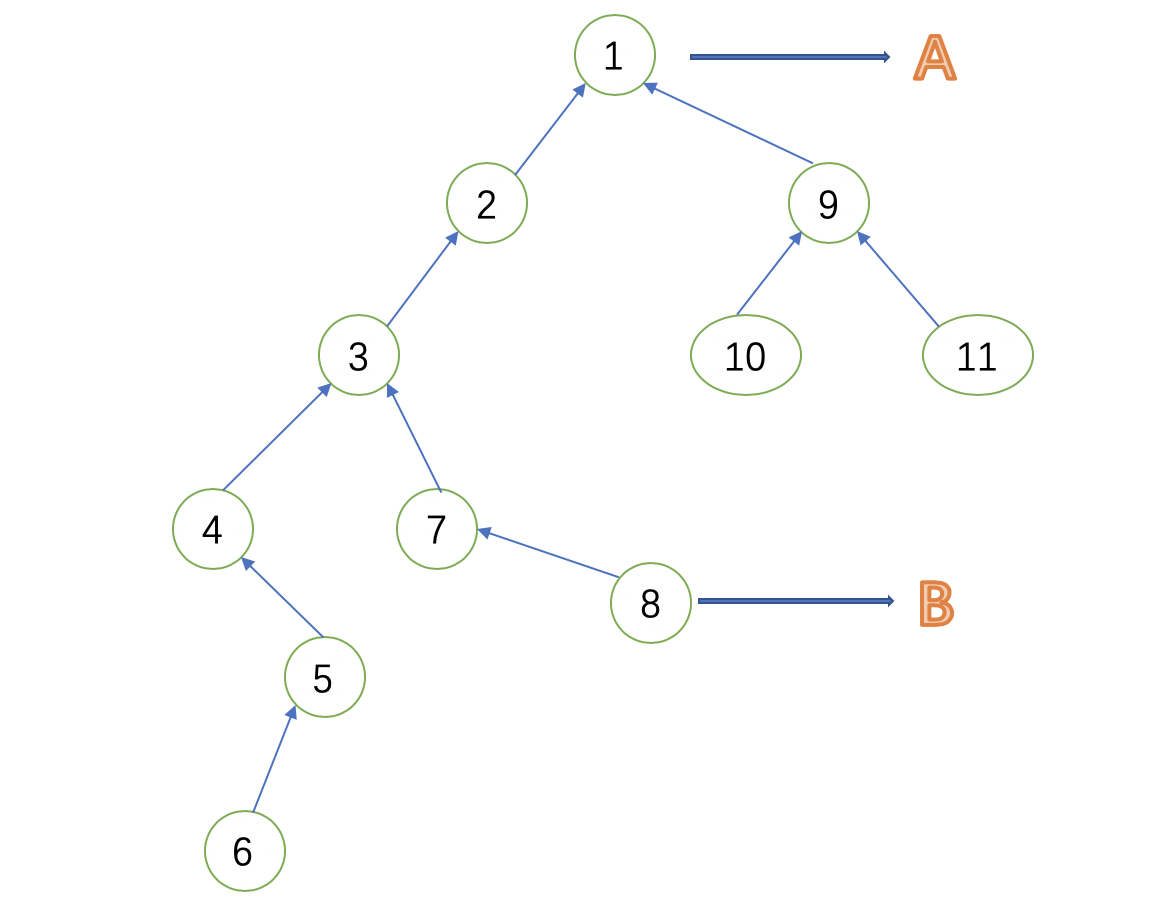
\includegraphics[width=0.6\textwidth]{3.png}
  
\begin{tikzpicture}
%\tikzset{grow'=right,level distance=32pt}
%\tikzset{execute at begin node=\strut}
%\tikzset{every tree node/.style={anchor=base west}}
\Tree
[.\node[fsn](n1){1};
  [.\node[sn]{2};
   [.\node[sn]{3};
    [.\node[sn]{4};
     [.\node[sn]{5};
      [.\node[sn]{6};]]]
    [.\node[sn]{7};
     [.\node[fsn](n8){8};]]] ]
  [.\node[sn]{9};
   [.\node[sn]{10};]
   [.\node[sn]{11};]
   [.\node[sn]{12};]]
]
\node (a) at ($(n1.east) + (1, 0)$) {A};
\node (b) at ($(n8.east) + (1, 0)$) {B};
\draw [->, >=stealth', color=blue] (n1) -- (a);
\draw [->, >=stealth', color=blue] (n8) -- (b);

\end{tikzpicture}

	\caption{Updating a path}
	\label{fig:2}
\end{figure}

We use the bracket sequence to handle this problem. A bracket sequence is to
record each node twice in the pre-order traversal, one for enter and one for
exit, called left bracket and right bracket respectively. For Figure~\ref{fig:2}, the bracket sequence is
$$1,2,3,4,5,6,6,5,4,7,8,8,7,3,2,9,10,10,11,11,12,12,9,1$$

For a direct path starts from $u$ and ends at $v$, define the path's {\em bracket interval} to be indexed from $v.leftbracket$ to $u.leftbreacket$. The following observation shows the property of the bracket interval:
\begin{observation}
Given a direct path, for any node that does not lie on the path, it occur twice or does not occur in the path's bracket interval. For any node that lies on the path, it occur exactly once in the path's bracket interval. Moreover, only the node’s first appearance lies in the interval.
\end{observation}
For example, suppose the path from 8 to 1 is to be updated, its bracket interval is $1,2,3,4,5,6,6,5,4,7,8$ (index 1-11). Nodes 4,5,6,11,12 do not lie on the path, so they occur twice or do not occur in the interval. Nodes 1,2,3,7,8 lie in the path, so they occur once in the interval. 

We then define an array $s[]$ for recording the so-called ``score" of the bracket sequence. Given a path where the nodes' lost voting powers need to add some value, we add that value into the scores of the path's bracket interval. Then for a node's  lost voting power, we can compute it by
 $$s[node.leftbracket]-s[node.rightbracket]$$
 The reason is that, when we increase the score, only the nodes on the path increase their lost voting powers (only the leftbracket increases). For a node outside the path, the scores either does not change or both its leftbraket and rightbracket increase by the same value, thus the lost voting power does not change.

We construct another interval tree with respect to the bracket sequence  and maintain the score, recorded in the variable $lazy_2[]$ of leaf nodes. The function $update2()$ gives the implementation.
\begin{algorithm}
	\textbf{procedure} $update2(int~L,int ~R, int~l, int~r, int~k, int~v)$
	\hrule
	\eIf {$L=l$ and $R=r$}
	{
       $lazy_2[k] \rightarrow lazy_2[k]+v$
	}
	{
		$int~m \leftarrow (l+r)/2$\;
		$lazy_2[2k] \rightarrow lazy_2[2k]+lazy_2[k]$\;
		$lazy_2[2k+1]\rightarrow lazy_2[2k+1]+lazy_2[k]$\;
		$lazy_2[k] \leftarrow 0$
			{\color{gray}
		//pass down the lazy-tag}\;
		\If {$L \leq m$}{$update2(L,\min\{m,R\},l,m,2k,v)$}
		\If {$R>m$}{$update2(\max\{m+1,L\},R,m+1,r,2k+1,v)$}
    }
\end{algorithm}
\begin{itemize}
	\item {\em update2(node.leftbracket,node.leftbracket,1,2n,1,0)} finds the score of the node's leftbracket. Similar for the rightbracket. 
	\item {\em update2(parent.leftbracket, node.leftbracket,1,2n,1,t)} update the score of the bracket interval of the path from the voter to its nearest parent.
\end{itemize}
So far our algorithm is introduced. In the next section we prove some theorems.